\documentclass[oneside]{book}

\usepackage[utf8]{inputenc}
\usepackage[a4paper]{geometry}
\usepackage[english]{babel}
\usepackage{cancel}
\usepackage{quotchap}
\usepackage{amsmath}
\usepackage{amssymb}
\usepackage{amsthm}
\usepackage{appendix}
\usepackage{array}
\usepackage{marvosym}
\usepackage[hidelinks]{hyperref}
\usepackage{color}
\usepackage[table]{xcolor}
\usepackage{amsthm}
\usepackage{graphicx}
\usepackage{polynom}
\usepackage{braket}
\usepackage{fontawesome}
\usepackage{mathtools}
\usepackage{tikz}
\usepackage{tkz-euclide}
\usepackage[most]{tcolorbox}
\usepackage{pgfplots}
\usepackage{multicol}
\usepgfplotslibrary{polar}
\usepgflibrary{shapes.geometric}
\usetikzlibrary{calc}
\pgfplotsset{def/.append style={axis x line=middle, axis y line=middle, xlabel={\(x\)}, ylabel={\(y\)}, axis equal}}
\pgfplotsset{compat=1.17}
\graphicspath{{./images/}}
\usetikzlibrary{fit,shapes}
\usetikzlibrary{graphs}

\DeclareMathOperator{\arcsec}{arcsec}
\DeclareMathOperator{\arccot}{arccot}
\DeclareMathOperator{\arccsc}{arccsc}
\DeclarePairedDelimiter{\ceil}{\lceil}{\rceil}
\DeclarePairedDelimiter{\floor}{\lfloor}{\rfloor}

\usepackage{fix-cm} 
\makeatletter
\newcommand\HUGE{\@setfontsize\Huge{50}{60}} 
\makeatother

\newcommand{\subsubsubsection}[1]{\paragraph{#1}\mbox{}\\}
\newcommand*{\?}{\stackrel{?}{=}}
\newcommand*{\dd}{\,\text{d}}
\newcommand*{\thus}{.^..}
%\renewcommand*{\and}{\wedge}
%\renewcommand*{\or}{\vee}
\newcommand*{\curl}{\text{curl\,}}
\newcommand*{\range}{\text{range\,}}
\renewcommand*{\div}{\text{div\,}}
\newcommand*{\Difficulty}{\Radioactivity}
%\newcommand*{\Difficulty}{\Frowny}
\newcommand*{\Stop}{\Stopsign}
\newcommand*{\DOTHISLATER}{\begin{center}\Stop\Stop\Stop\Stop\Stop\Stop\Stop\Stop\Stop\Stop\Stop\Stop\Stop\Stop\Stop\end{center}}
\newcommand*{\laplace}[2][]{\mathcal{L}^{#1}\left\{#2\right\}}
\newcommand*{\powerset}[1]{\mathcal{P}\left(#1\right)}
\renewcommand*{\vec}[1]{\overset{_{\rightharpoonup}}{#1}}
\renewcommand*{\bar}[1]{\overline{#1}}
\renewcommand*{\gcd}[2]{\text{gcd}\left(#1,#2\right)}
%\renewcommand*{\vec}[1]{\mathbf{#1}}
\newcommand*{\nin}{\notin}
\newcommand*{\nequiv}{\not\equiv}
\newcommand*{\Span}{\text{span\,}}
\newcommand*{\proj}{\text{proj\,}}
\newcommand*{\rank}{\text{rank\,}}
\newcommand*{\nullity}{\text{nullity\,}}
\newcommand*{\trace}{\text{trace\,}}
\newcommand*{\iprod}[2]{\left\langle #1,#2\right\rangle}


\usepackage{sfmath}
\renewcommand{\familydefault}{\sfdefault}

% \renewcommand*{\qedsymbol}{\(\blacksquare\)}

\newtcbtheorem[number within=section]{definition}{Definition}{
                lower separated=false,
                breakable,
                before skip=0.5cm,
                colback=white,
                colframe=black,fonttitle=\bfseries,
                colbacktitle=black,
                coltitle=white,
                enhanced,
                attach boxed title to top left={yshift=-0.1in,xshift=0.15in},
                }{def}
                
\newtcbtheorem[number within=section]{example}{Example}{
                lower separated=false,
                breakable,
                before skip=0.5cm,
                colback=gray!15,
                colframe=white!10!black,fonttitle=\bfseries,
                colbacktitle=black,
                coltitle=white,
                enhanced,
                attach boxed title to top left={yshift=-0.1in,xshift=0.15in},
                }{exa}
                
\newtcbtheorem[number within=section]{exercise}{Exercise}{
                lower separated=false,
                breakable,
                before skip=0.5cm,
                colback=gray!15,
                colframe=white!10!black,fonttitle=\bfseries,
                colbacktitle=black,
                coltitle=white,
                enhanced,
                attach boxed title to top left={yshift=-0.1in,xshift=0.15in},
                }{exe}
                
\newtcbtheorem[number within=section]{theorem}{Theorem}{
                lower separated=false,
                breakable,
                before skip=0.5cm,
                colback=white,
                colframe=black,fonttitle=\bfseries,
                colbacktitle=black,
                coltitle=white,
                enhanced,
                attach boxed title to top left={yshift=-0.1in,xshift=0.15in},
                }{thm}
                
\newtcbtheorem[number within=section]{solution}{Solution}{
                lower separated=false,
                before skip=0.5cm,
                breakable,
                colback=white,
                colframe=black,fonttitle=\bfseries,
                colbacktitle=black,
                coltitle=white,
                enhanced,
                attach boxed title to top left={yshift=-0.1in,xshift=0.15in},
                }{sol}
            
\usepackage{listings}
\usepackage{xcolor}

% Configuration for Syntax Highlighting
\definecolor{codegreen}{rgb}{0,0.6,0}
\definecolor{codegray}{rgb}{0.5,0.5,0.5}
\definecolor{codepurple}{rgb}{0.58,0,0.82}
\definecolor{backcolour}{rgb}{0.95,0.95,0.92}
\definecolor{bggray}{gray}{0.9}

\renewcommand{\ttdefault}{pcr}
\lstdefinestyle{code}{
    backgroundcolor=\color{bggray},   
    commentstyle=\color{gray},
    keywordstyle=\bfseries,
    morekeywords={def},
    numberstyle=\tiny\color{black},
    %stringstyle=\color{codepurple},
    basicstyle=\ttfamily\footnotesize,
    breakatwhitespace=false,         
    breaklines=true,                 
    captionpos=b,                    
    keepspaces=true,                 
    numbers=left,                    
    numbersep=5pt,                  
    showspaces=false,                
    showstringspaces=false,
    showtabs=false,                  
    tabsize=2
}

\lstset{style=code}

\newenvironment{code}{\fontfamily{lmtt}\selectfont}{\par}
\geometry{left=2.54cm}
\geometry{right=2.54cm}
\colorlet{chaptergrey}{black}

\title{

    \rule{15cm}{1.6pt}\vspace*{-\baselineskip}\vspace*{2pt}
    \rule{15cm}{0.4pt}
	
	\vspace{0.75\baselineskip}
		
	\Huge{MATH1300: CALCULUS I\\\vspace{3mm}}

	\rule{15cm}{0.4pt}\vspace*{-\baselineskip}\vspace{3.2pt}
	\rule{15cm}{1.6pt}

}

\author{ADITHYA BHASKARA\\\\\vspace{1em}\small{COURSE COORDINATORS: HARRISON STALVEY \& CHRISTOPHER EBLEN}\\\vspace{1em}\small{TEXTBOOK: JAMES STEWART}}

\date{}

\begin{comment}
\usepackage{draftwatermark}

\SetWatermarkText{Draft: \today}
\SetWatermarkColor[gray]{0.5}
\SetWatermarkFontSize{1cm}
\SetWatermarkAngle{90}
\SetWatermarkHorCenter{20cm}
\end{comment}

\begin{document}

\begin{center} 
    \begin{minipage}{\textwidth}
        \maketitle
        \begin{center}
        \begin{tabular}{c}
            UNIVERSITY OF COLORADO BOULDER \\
            \hline \\
        \end{tabular}
        \\
        
\includegraphics[scale=0.2]{Graphics/CU.png}
        \end{center}
    \end{minipage}
\end{center}

\vfill
\rightline{\textbf{EDITION 1}}
\frontmatter

\begin{center}
    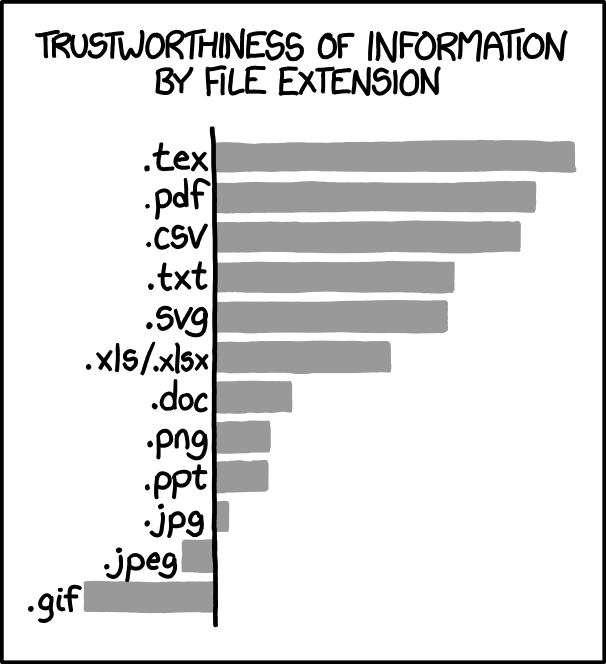
\includegraphics[scale=1.5, width=\textwidth]{Graphics/latex.png}
\end{center}

\pagebreak

\tableofcontents

\setcounter{tocdepth}{4}
\setcounter{secnumdepth}{4}

\pagebreak

\chapter*{Preface}
\addcontentsline{toc}{chapter}{Preface}

To the interested reader,
\\
\\
This document is a compilation of notes taken during the Spring 2023 semester for MATH1300: Calculus I at the University of Colorado Boulder during the author's tenure as a learning assistant for the course. The course used \textit{Calculus -- Concepts and Contexts}\footnote{Stewart, J. (2010). \textit{Calculus -- Concepts and Contexts} (4th ed.). Cengage.} by James Stewart as its primary text and was coordinated by Harrison Stalvey and Christopher Eblen. Additionally, in creating these notes, the author used \textit{Calculus} by Ron Larson and Bruce Edwards. As such, many theorems, definitions, and examples may be quoted or derived from the aforementioned books. The section names will follow Stewart's book exactly.
\\
\\
The author would like to provide the following resources for students currently taking a Calculus I course:
\begin{enumerate}
    \item \href{https://tutorial.math.lamar.edu/classes/calci/calci.aspx}{Paul's \textit{Online Math Notes} for Calculus I at Lamar University.}
    \item \href{https://youtube.com/playlist?list=PLF797E961509B4EB5}{Professor Leonard's YouTube Calculus I Lectures.}
    \item \href{https://www.youtube.com/watch?v=WUvTyaaNkzM&list=PLZHQObOWTQDMsr9K-rj53DwVRMYO3t5Yr}{3Blue1Brown's \textit{Essence of Calculus}.}
\end{enumerate}
\vphantom
\\
\\
Theorems, definitions, and examples may be quoted or derived from the aforementioned resources as well.
\\
\\
While much effort has been put in to remove typos and mathematical errors, it is very likely that some errors, both small and large, are present. If an error needs to be resolved, please contact Adithya Bhaskara at \href{mailto:adithya.bhaskara@colorado.edu}{adithya.bhaskara@colorado.edu}.
\\
\\
\rightline{Best Regards,}
\rightline{Adithya Bhaskara}
\vfill
\rightline{\textbf{REVISED: \today}}

\mainmatter

\begin{savequote}

\end{savequote}
\chapter{Functions and Models} \label{chapter:funcmod}

    \section{Week 1: January 16 -- January 20}

\begin{savequote}

\end{savequote}
\chapter{Limits and Derivatives} \label{chapter:limder}

    \section{Week 1: January 16 -- January 20}

    \subsection{The Tangent and Velocity Problems}

        We seek to find the equation of a line \(L(x)\) that touches the curve created by \(f(x)\) at only one point \((x_0,f(x_0))\) \textit{near} \(x=x_0\). To better visualize this, imagine \(f(x)\) to be the path a car drives. We seek to find the line that the car would follow if the driver immediately jerked the wheel to the straight position at some point \(x_0\). Consider the following graphs.
        \begin{center}
            \begin{tabular}{cc}
                \begin{tikzpicture}
                    \begin{axis} [def]
                        \addplot [domain=-10:10, restrict y to domain=-10:10] {x^3-x+5}; 
                        \addplot [domain=-10:10, restrict y to domain=-10:10] {2*x+3}; 
                        \addplot [only marks] table {
						1 5
						};
                    \end{axis}
                \end{tikzpicture}
                &
                \begin{tikzpicture}
                    \begin{axis} [def]
                        \addplot [domain=-5:5, restrict y to domain=-10:10] {-3/(x^2-4)}; 
                        \addplot [domain=-5:5, restrict y to domain=-10:10] {2*x/3+1/3}; 
                        \addplot [only marks] table {
						1 1
						};
                    \end{axis}
                \end{tikzpicture}
            \end{tabular}
        \end{center}
        \pagebreak
        \vphantom
        \\
        \\
        While it can be easy to sketch this line, finding the equation is certainly not trivial. The difficulty lies in finding the slope \(m\) of the line. Then, the equation is given by the point-slope formula. That is,
        \begin{equation*}
            L(x)-f(x_0)=m(x-x_0)\implies L(x)=f(x_0)+m(x-x_0).
        \end{equation*}
        We only have one point, \(x_0\) at our disposal, yet we need two points to calculate the slope. We will choose our second point, \(x_1\), to be somewhere near \(x_0\) to approximate the slope. Recall the slope of the line formed by \(x_0\) and \(x_1\), or equivalently, the average slope of \(f(x)\) on the interval \([x_0,x_1]\) is
        \begin{equation*}
            \bar{m}=\frac{f(x_1)-f(x_0)}{x_1-x_0}.
        \end{equation*}
        Our method will be to gradually move the point \(x_1\) closer to \(x_0\) until the two points are indistinguishable from each other. The two points will be \textit{arbitrarily close} to each other. Then, the slope between the points will be the slope of the tangent line. The following graphs will visualize this method and find a tangent line for \(f(x)=x^2\) at \((1,1)\).
        \begin{center}
            \begin{tabular}{cccc}
                \begin{tikzpicture}[scale=0.5]
                    \begin{axis} [def]
                        \addplot [domain=-10:10, restrict y to domain=-10:10] {x^2}; 
                        \addplot [domain=-10:10, restrict y to domain=-10:10, dashed] {8*(x-1)/-4+1}; 
                        \addplot [only marks] table {
						1 1
                        -3 9
						};
                    \end{axis}
                \end{tikzpicture}
                &
                \begin{tikzpicture}[scale=0.5]
                    \begin{axis} [def]
                        \addplot [domain=-10:10, restrict y to domain=-10:10] {x^2}; 
                        \addplot [domain=-10:10, restrict y to domain=-10:10, dashed] {3*(x-1)/-3+1}; 
                        \addplot [only marks] table {
						1 1
                        -2 4
						};
                    \end{axis}
                \end{tikzpicture}
                &
                \begin{tikzpicture}[scale=0.5]
                    \begin{axis} [def]
                        \addplot [domain=-10:10, restrict y to domain=-10:10] {x^2}; 
                        \addplot [domain=-10:10, restrict y to domain=-10:10, dashed] {1.25*(x-1)/-2.5+1}; 
                        \addplot [only marks] table {
						1 1
                        -1.5 2.25
						};
                    \end{axis}
                \end{tikzpicture}
                &
                \begin{tikzpicture}[scale=0.5]
                    \begin{axis} [def]
                        \addplot [domain=-10:10, restrict y to domain=-10:10] {x^2}; 
                        \addplot [domain=-10:10, restrict y to domain=-10:10, dashed] {-1*(x-1)/-1+1}; 
                        \addplot [only marks] table {
						1 1
                        0 0
						};
                    \end{axis}
                \end{tikzpicture}
                \\
                \begin{tikzpicture}[scale=0.5]
                    \begin{axis} [def]
                        \addplot [domain=-10:10, restrict y to domain=-10:10] {x^2}; 
                        \addplot [domain=-10:10, restrict y to domain=-10:10] {2*(x-1)+1}; 
                        \addplot [only marks] table {
						1 1
						};
                    \end{axis}
                \end{tikzpicture}
                &
                \begin{tikzpicture}[scale=0.5]
                    \begin{axis} [def]
                        \addplot [domain=-10:10, restrict y to domain=-10:10] {x^2}; 
                        \addplot [domain=-10:10, restrict y to domain=-10:10, dashed] {1.25*(x-1)/0.5+1}; 
                        \addplot [only marks] table {
						1 1
                        1.5 2.25
						};
                    \end{axis}
                \end{tikzpicture}
                &
                \begin{tikzpicture}[scale=0.5]
                    \begin{axis} [def]
                        \addplot [domain=-10:10, restrict y to domain=-10:10] {x^2}; 
                        \addplot [domain=-10:10, restrict y to domain=-10:10, dashed] {3*(x-1)+1}; 
                        \addplot [only marks] table {
						1 1
                        2 4
						};
                    \end{axis}
                \end{tikzpicture}
                &
                \begin{tikzpicture}[scale=0.5]
                    \begin{axis} [def]
                        \addplot [domain=-10:10, restrict y to domain=-10:10] {x^2}; 
                        \addplot [domain=-10:10, restrict y to domain=-10:10, dashed] {8*(x-1)/2+1}; 
                        \addplot [only marks] table {
						1 1
                        3 9
						};
                    \end{axis}
                \end{tikzpicture}
            \end{tabular}
        \end{center}
        \vphantom
        \\
        \\
        We can say that the slope of the tangent line is the limit of the slopes of the secant lines \(\bar{m}\) as \(x_1\) approaches \(x_0\). That is,
        \begin{equation*}
            m=\lim_{x_1\to x_0}\frac{f(x_1)-f(x_0)}{x_1-x_0}.
        \end{equation*}
        Many texts will instead use
        \begin{equation*}
            m=\lim_{x\to a}\frac{f(x)-f(a)}{x-a}
        \end{equation*}
        to mean the same thing--the slope of the tangent line of \(f(x)\) at \((x_0,f(x_0))\), or equivalently, \((a,f(a))\). That means \(L(x)\) is given by
        \begin{equation*}
            L(x)=f(x_0)+\lim_{x_1\to x_0}\frac{f(x_1)-f(x_0)}{x_1-x_0}(x-x_0).
        \end{equation*}
        \\
        \\
        The specific answer to our question about \(f(x)=x^2\) is not important for now, but the process described certainly is. We will defer the computation to a later section.
        \pagebreak
        \\
        \\
        We will now turn to the velocity problem. Speedometers in cars are useful, as they help the driver keep track of the velocity they are going at very moment \(t_0\) in their journey. How is this instantaneous velocity defined, given that the average velocity of an object is given by its change in position divided by the elapsed time? The notion of ``elapsed time'' seems to require two distinct timestamps to measure. Again, the difficulty lies in that we are only given one value, \(t_0\), to determine the instantaneous velocity at. Suppose we are given a position function \(x(t)\). Then, the time elapsed between \(t_1\) and \(t_0\) is \(t_1-t_0\). The change in position is \(x(t_1)-x(t_0)\), meaning that the average velocity on the interval \([t_0,t_1]\) is
        \begin{equation*}
            \bar{v}=\frac{x(t_1)-x(t_0)}{t_1-t_0}.
        \end{equation*}
        To get a better approximation of the instantaneous velocity at \(t_0\), we can decrease the elapsed time by choosing \(t_1\) near \(t_0\) and take the limit as \(t_1\) approaches \(t_0\). Then, we have
        \begin{equation*}
            v=\lim_{t_1\to t_0}\frac{x(t_1)-x(t_0)}{t_1-t_0}.
        \end{equation*}
        Similarly, some texts may instead use
        \begin{equation*}
            v=\lim_{t\to a}\frac{x(t)-x(a)}{t-a}.
        \end{equation*}
        We will end with the notion that your car's speedometer uses the above technique with extremely small time intervals.

    \pagebreak

    \subsection{The Limit of a Function}

        To solve the problems described in the previous section, we must learn to evaluate limits. With limits, we care not about the value of a function at some value \(x=a\). We instead care about how the function \textit{behaves} close to that value. Consider the following definition.
        \begin{definition}{\Stop\,\,Limits}{limits}

            We write
            \begin{equation*}
                \lim_{x\to a}f(x)=L
            \end{equation*}
            and say ``the limit of \(f(x)\), as \(x\) approaches \(a\)'' is \(L\) if and only if we can make the values of \(f(x)\) arbitrarily close to \(L\) by taking \(x\) to be sufficiently close to \(a\), on either side, while \(x\neq a\).
            
        \end{definition}
        \vphantom
        \\
        \\
        The above definition means that the values of \(f(x)\) get closer and closer to \(L\) as \(x\) gets closer and closer to \(a\), on either side. If this is not true, the limit does not exist. We will often abbreviate ``does not exist'' to ``DNE.'' The definition makes clear that the value of \(f(a)\) is irrelevant. We care only about the value of \(f(x)\) for \(x\) near \(a\). Consider the following graphs.
        \begin{center}
            \begin{tabular}{ccc}
                \begin{tikzpicture}[scale=0.6]
                    \begin{axis} [def]
                        \addplot [domain=0:5, restrict y to domain=0:5] {x^3}; 
                        \addplot [domain=-5:0, restrict y to domain=-5:0] {x}; 
                        \addplot [only marks, mark=o] table {
                        0 0
                        };
                    \end{axis}
                \end{tikzpicture}
                &
                \begin{tikzpicture}[scale=0.6]
                    \begin{axis} [def]
                        \addplot [domain=0:5, restrict y to domain=0:5] {x^3}; 
                        \addplot [domain=-5:0, restrict y to domain=-5:0] {x}; 
                    \end{axis}
                \end{tikzpicture}
                &
                \begin{tikzpicture}[scale=0.6]
                    \begin{axis} [def]
                        \addplot [domain=0:5, restrict y to domain=0:5] {x^3}; 
                        \addplot [domain=-5:0, restrict y to domain=-5:0] {x}; 
                        \addplot [only marks, mark=o] table {
                        0 0
                        };
                        \addplot [only marks] table {
                        0 2
                        };
                    \end{axis}
                \end{tikzpicture}
            \end{tabular}
        \end{center}
        \vphantom
        \\
        \\
        At \(x=0\), all of the above graphs have different behavior; however, the limit, as \(x\) approaches \(0\) is the same regardless: \(0\). To estimate a limit as \(x\) approaches \(a\) with a graph of \(f(x)\), simply use a pen or other writing utensil to trace the graph toward \(x=a\), from both sides, and record the value that the function approaches, if there is one.
        \pagebreak
        \\
        \\
        We can often estimate the limit \(\lim_{x\to a}f(x)\) by creating a table of values for \(x\) and \(f(x)\) for \(x\) near \(a\). Consider the following examples.
        \begin{example}{\Difficulty\,\Difficulty\,\,Estimating a Limit 1}{estlim1}
            
            Estimate the limit
            \begin{equation*}
                \lim_{x\to 0}\frac{\sin x}{x}.
            \end{equation*}
            Consider the following table.
            \begin{center}
                \begin{tabular}{|cc|}
                    \hline
                    \(x\) & \(f(x)\) \\
                    \hline
                    \(-1\) & \(0.84147098\) \\
                    \(-0.1\) & \(0.99833417\) \\
                    \(-0.01\) & \(0.99998333\) \\
                    \(0.01\) & \(0.99998333\) \\
                    \(0.1\) & \(0.99833417\) \\
                    \(1\) & \(0.84147098\) \\
                    \hline
                \end{tabular}
            \end{center}
            \vphantom
            \\
            \\
            Therefore, we estimate that 
            \begin{equation*}
                \lim_{x\to 0}\frac{\sin x}{x}=1
            \end{equation*}

        \end{example}
        \begin{example}{\Difficulty\,\Difficulty\,\,Estimating a Limit 2}{estlim2}
            
            Estimate the limit
            \begin{equation*}
                \lim_{x\to 0}\frac{1-\cos x}{x}.
            \end{equation*}
            Consider the following table.
            \begin{center}
                \begin{tabular}{|cc|}
                    \hline
                    \(x\) & \(f(x)\) \\
                    \hline
                    \(-1\) & \(-0.45969769\) \\
                    \(-0.1\) & \(-0.049958347\) \\
                    \(-0.01\) & \(-0.0049999583\) \\
                    \(0.01\) & \(0.0049999583\) \\
                    \(0.1\) & \(0.049958347\) \\
                    \(1\) & \(0.45969769\) \\
                    \hline
                \end{tabular}
            \end{center}
            Therefore, we estimate that 
            \begin{equation*}
                \lim_{x\to 0}\frac{1-\cos x}{x}=0
            \end{equation*}

        \end{example}
        \pagebreak
        \begin{example}{\Difficulty\,\Difficulty\,\,Estimating a Limit 3}{estlim3}
            
            Estimate the limit
            \begin{equation*}
                \lim_{x\to 0}\sin\left(\frac{1}{x}\right)
            \end{equation*}
            Consider the following table.
            \begin{center}
                \begin{tabular}{|cc|}
                    \hline
                    \(x\) & \(f(x)\) \\
                    \hline
                    \(-1\) & \(0\) \\
                    \(-0.1\) & \(0\) \\
                    \(-0.01\) & \(0\) \\
                    \(0.01\) & \(0\) \\
                    \(0.1\) & \(0\) \\
                    \(1\) & \(0\) \\
                    \hline
                \end{tabular}
            \end{center}
            Therefore, we estimate that 
            \begin{equation*}
                \lim_{x\to 0}\sin\left(\frac{1}{x}\right)=0.
            \end{equation*}
            However, this is wrong, and a good reminder to be cautious while estimating. Consider the following graph of \(\sin\left(\frac{1}{x}\right)\).
            \begin{center}
                \begin{tikzpicture}
                    \begin{axis} [def]
                        \addplot [domain=-pi:pi, samples=1000, restrict y to domain=-5:5] {sin(deg(1/x))}; 
                    \end{axis}
                \end{tikzpicture}
            \end{center}
            \vphantom
            \\
            \\
            We see that as \(x\) approaches zero, it is not true that \(\sin\left(\frac{1}{x}\right)\) approaches zero. Instead, the function oscillates between \(-1\) and \(1\) infinitely many times. Therefore
            \begin{equation*}
                \lim_{x\to 0}\sin\left(\frac{1}{x}\right)\text{ DNE}.
            \end{equation*}

        \end{example}
        \pagebreak
        \vphantom
        \\
        \\
        Often, it is useful to only scrutinize the limiting behavior of one side of some \(a\) instead of looking at both sides. Consider the following definition and related theorem.
        \begin{definition}{\Stop\,\,One-Sided Limits}{onesidedlimits}

            We write
            \begin{equation*}
                \lim_{x\to a^-}f(x)=L
            \end{equation*}
            and say ``the left-hand limit of \(f(x)\) as \(x\) approaches \(a\)'' is \(L\) if and only if we can make the values of \(f(x)\) arbitrarily close to \(L\) by taking \(x\) to be sufficiently close to \(a\) and \(x<a\).
            \\
            \\
            We write
            \begin{equation*}
                \lim_{x\to a^+}f(x)=L
            \end{equation*}
            and say ``the right-hand limit of \(f(x)\) as \(x\) approaches \(a\)'' is \(L\) if and only if we can make the values of \(f(x)\) arbitrarily close to \(L\) by taking \(x\) to be sufficiently close to \(a\) and \(x>a\).

        \end{definition}
        \begin{theorem}{\Stop\,\,The Relationship Between Limits and One-Sided Limits}{limonelim}
            
            For some function \(f(x)\), \(\lim_{x\to a}f(x)=L\) if and only if \(\lim_{x\to a^-}f(x)=L=\lim_{x\to a^+}f(x)\).

        \end{theorem}
        \pagebreak
        \vphantom
        \\
        \\
        Consider the following example.
        \begin{example}{\Difficulty\,\Difficulty\,\,Determining Limits Graphically}{graphlim}
            
            Let \(f(x)\) be defined by the following graph.
            \begin{center}
                \begin{tikzpicture}[scale=1]
                    \begin{axis} [def]
                        \addplot [domain=0:5, restrict y to domain=0:5] {x^3}; 
                        \addplot [domain=-2:0, restrict y to domain=0:5] {x^2}; 
                        \addplot [domain=-5:-2, restrict y to domain=-5:0] {x}; 
                        \addplot [only marks, mark=o] table {
                        -2 4
                        0 0
                        -2 -2
                        };
                        \addplot [only marks] table {
                        0 2
                        };
                    \end{axis}
                \end{tikzpicture}
            \end{center}
            \vphantom
            \\
            \\
            Find the quantities
            \begin{equation*}
                \lim_{x\to -2^-}f(x),\quad \lim_{x\to -2^+}f(x),\quad \lim_{x\to 0^-}f(x),\quad \lim_{x\to 0^+}f(x),
            \end{equation*}
            and
            \begin{equation*}
                \lim_{x\to -2}f(x),\quad \lim_{x\to 0}f(x).
            \end{equation*}
            We see that
            \begin{equation*}
                \lim_{x\to -2^-}f(x)=-2,\quad \lim_{x\to -2^+}f(x)=4,\quad \lim_{x\to 0^-}f(x)=0,\quad \lim_{x\to 0^+}f(x)=0,
            \end{equation*}
            so
            \begin{equation*}
                \lim_{x\to -2}f(x)\text{ DNE},\quad \lim_{x\to 0}f(x)=0.
            \end{equation*}

        \end{example}

\pagebreak

\section{Week 2: January 23 -- January 27}

    \subsection{Calculating Limits Using the Limit Laws}

        Consider the following properties of limits.
        \begin{theorem}{\Stop\,\,Limit Laws}{limlaws}

            Let \(a\) and \(c\) be constants and let the limits \(\lim_{x\to a}f(x)\) and \(\lim_{x\to a}g(x)\) exist. Then,
            \begin{enumerate}
                \item \(\lim\limits_{x\to a}[f(x)\pm g(x)]=\lim\limits_{x\to a}f(x)\pm\lim\limits_{x\to a}g(x)\).
                \item \(\lim\limits_{x\to a}[cf(x)]=c\lim\limits_{x\to a}f(x)\).
                \item \(\lim\limits_{x\to a}[f(x)g(x)]=\lim\limits_{x\to a}f(x)\lim\limits_{x\to a}g(x)\).
                \item \(\lim\limits_{x\to a}\left[\frac{f(x)}{g(x)}\right]=\frac{\lim\limits_{x\to a}f(x)}{\lim\limits_{x\to a}g(x)}\) if \(\lim\limits_{x\to a}g(x)\neq0\).
                \item \(\lim\limits_{x\to a}c=c\).
                \item \(\lim\limits_{x\to a}x=a\).
            \end{enumerate}
            
        \end{theorem}
        \vphantom
        \\
        \\
        If we take the laws in Theorem \ref{thm:limlaws} for granted, we have the following consequences.
        \begin{theorem}{\Stop\,\,Derived Limit Laws}{derlimlaws}

            Let \(a\) and \(c\) be constants and let the limit \(\lim_{x\to a}f(x)\) exist. Let \(n\) be a positive integer. Then,
            \begin{enumerate}
                \item \(\lim\limits_{x\to a}[f(x)]^n=\left[\lim\limits_{x\to a}f(x)\right]^n\).
                \item \(\lim\limits_{x\to a}\sqrt[n]{f(x)}=\sqrt[n]{\lim\limits_{x\to a}f(x)}\).
                \item \(\lim\limits_{x\to a}x^n=a^n\).
                \item \(\lim\limits_{x\to a}\sqrt[n]{x}=\sqrt[n]{a}\).
            \end{enumerate}
            
        \end{theorem}
        \vphantom
        \\
        \\
        Theorems \ref{thm:limlaws} and \ref{thm:derlimlaws} allow us to claim the following.
        \begin{theorem}{\Stop\,\,Direct Substitution}{dirsub}

            If \(f\) is a polynomial or rational function and \(a\) is in the domain of \(f\),
            \begin{equation*}
                \lim_{x\to a}f(x)=f(a).
            \end{equation*}
            
        \end{theorem}
        \vphantom
        \\
        \\
        There exist other functions with the property described in Theorem \ref{thm:dirsub}, but we will postpone their discussion to a later section.
        \pagebreak
        \\
        \\
        Consider the following examples.
        \begin{example}{\Difficulty\,\Difficulty\,\,Direct Substitution 1}{dirsub1}

            Evaluate \(\lim_{x \to 2}(x^3+2x^2-11x-7)\).
            \\
            \\
            We see that
            \begin{align*}
                \lim_{x \to 2}(x^3+2x^2-11x-7)&=(2)^3+2(2)^2-11(2)-7 \\
                &=8+8-22-7 \\
                &=-13.
            \end{align*}

        \end{example}
        \begin{example}{\Difficulty\,\Difficulty\,\,Direct Substitution 2}{dirsub2}
            
            Evaluate \(\lim_{x \to 3}\frac{2x}{x-4}\).
            \\
            \\
            We see that
            \begin{align*}
                \lim_{x \to 3}\frac{2x}{x-4}&=\frac{2(3)}{(3)-4} \\
                &=-6.
            \end{align*}

        \end{example}
        \vphantom
        \\
        \\
        Most of the time, direct substitution will not work, but it is often beneficial to try it before trying anything else. It will certainly not work when the function is not defined at the value the limit is being evaluated at, and it is beneficial to use caution when considering piecewise functions. Consider the following theorem.
        \begin{theorem}{\Stop\,\,Limit Equivalence of Two Functions}{limequivtwofunc}
            
            If \(f(x)=r(x)\) whenever \(x\neq a\),
            \begin{equation*}
                \lim_{x\to a}f(x)=\lim_{x\to a }r(x).
            \end{equation*}

        \end{theorem}
        \vphantom
        \\
        \\
        When given a function \(f(x)\) where direct substitution fails, we will find a function \(r(x)\) such that \(f(x)=r(x)\) whenever \(x\neq a\) and compute \(\lim_{x\to a}r(x)\). Then, we will use Theorem \ref{thm:limequivtwofunc} to conclude that \(\lim_{x\to a}r(x)=\lim_{x\to a}f(x)\). This process is called removing a discontinuity.
        \pagebreak
        \\
        \\
        Consider the following examples.
        \begin{example}{\Difficulty\,\Difficulty\,\,Removing a Discontinuity 1}{remdiscont1}

            Evaluate \(\lim_{x\to -3}\frac{x^2+6x+6}{x+3}\). 
            \\
            \\
            Let \(f(x)=\frac{x^2+6x+6}{x+3}\). We note that direct substitution fails on \(f(x)\) since \(f(x)\) is not defined at \(x=-3\). We cannot use our limit laws since \(\lim_{x\to -3}(x+3)=0\). We must find \(r(x)\) such that \(r(x)=f(x)\) whenever \(x\neq -3\). Consider
            \begin{align*}
                f(x)&=\frac{x^2+5x+6}{x+3} \\
                &=\frac{(x+3)(x+2)}{x+3} \\
                &=x+2,\quad {x\neq -3}.
            \end{align*}
            Then \(r(x)=x+2=f(x)\), except at \(x=-3\); \(r(-3)=-1\) while \(f(-3)\) is not defined. Then we can apply direct substitution on \(r(x)\) to obtain
            \begin{align*}
                \lim_{x\to -3}\frac{x^2+6x+6}{x+3}&=\lim_{x\to -3}(x+2) \\
                &=-3+2 \\
                &=1.
            \end{align*}
        
        \end{example}
        \begin{example}{\Difficulty\,\Difficulty\,\,Removing a Discontinuity 2}{remdiscont2}

            Evaluate \(\lim_{x \to -5}\frac{x^3+5x^2}{x+5}\).
            \\
            \\
            Let \(f(x)=\frac{x^3+5x^2}{x+5}\). We note that direct substitution fails on \(f(x)\) since \(f(x)\) is not defined at \(x=-5\). We cannot use our limit laws since \(\lim_{x\to -5}(x+5)=0\). We must find \(r(x)\) such that \(r(x)=f(x)\) whenever \(x\neq -5\). Consider
            \begin{align*}
                f(x)&=\frac{x^3+5x^2}{x+5} \\
                &=\frac{x^2(x+5)}{x+5} \\
                &=x^2,\quad x\neq 5.
            \end{align*}
            Then \(r(x)=x^2=f(x)\), except at \(x=-5\); \(r(-5)=25\) while \(f(-5)\) is not defined. Then we can apply direct substitution on \(r(x)\) to obtain
            \begin{align*}
                \lim_{x \to -5}\frac{x^3+5x^2}{x+5}&=\lim_{x\to -5}x^2 \\
                &=25.
            \end{align*}
            
        \end{example}
        \begin{example}{\Difficulty\,\Difficulty\,\,Removing a Discontinuity 3}{remdiscont3}

            Evaluate \(\lim_{x \to 7}\frac{\sqrt{x+9}-4}{x-7}\).
            \\
            \\
            Let \(f(x)=\frac{\sqrt{x+9}-4}{x-7}\). We note that direct substitution fails on \(f(x)\) since \(f(x)\) is not defined at \(x=7\). We cannot use our limit laws since \(\lim_{x\to 7}(x-7)=0\). We must find \(r(x)\) such that \(r(x)=f(x)\) whenever \(x\neq 7\). Consider
            \begin{align*}
                f(x)&=\frac{\sqrt{x+9}-4}{x-7} \\
                &=\frac{\sqrt{x+9}-4}{x-7}\frac{\sqrt{x+9}+4}{\sqrt{x+9}+4} \\
                &=\frac{x+9-16}{(x-7)(\sqrt{x+9}+4)} \\
                &=\frac{1}{\sqrt{x+9}+4},\quad x\neq 7.
            \end{align*}
            Then \(r(x)=\frac{1}{\sqrt{x+9}+4}=f(x)\), except at \(x=7\); \(r(7)=\frac{1}{8}\) while \(f(7)\) is not defined. Then we can apply direct substitution on \(r(x)\) to obtain
            \begin{align*}
                \lim_{x \to 7}\frac{\sqrt{x+9}-4}{x-7}&=\lim_{x\to 7}\frac{1}{\sqrt{x+9}+4} \\
                &=\frac{1}{8}.
            \end{align*}
            
        \end{example}
        \begin{example}{\Difficulty\,\Difficulty\,\,Piecewise Functions and Direct Substitution}{piecewisedirsub}

            Let \(f(x)=\begin{cases} x+5 & x \neq 2 \\ e & x=2 \end{cases}\). Evaluate \(\lim_{x \to 2}f(x)\).
            \\
            \\
            If we try direct substitution, we may come to the conclusion that the desired limit is simply \(e\); however, this is not the case, as we can construct \(r(x)=x+5\) and note that \(r(x)=f(x)\) whenever \(x\neq 2\). Therefore,
            \begin{align*}
                \lim_{x \to 2}f(x)&=\lim_{x \to 2}r(x) \\
                &=2+5 \\
                &=7.
            \end{align*}
            
        \end{example}
        \pagebreak
        \vphantom
        \\
        \\
        For piecewise functions in particular, it is often beneficial to compute the one-sided limits when trying to find a limit. Consider the following examples.
        \begin{example}{\Difficulty\,\Difficulty\,\,Piecewise Functions and One-Sided Limits 1}{piecewiseonesided1}

            Let \(f(x)=\begin{cases} x+5 & x \neq 2 \\ e & x=2 \end{cases}\). Evaluate \(\lim_{x \to 2}f(x)\).
            \\
            \\
            For \(x>2\), \(f(x)=x+5\). Therefore, \(\lim_{x\to 2^+}f(x)=7\). Similarly, for \(x<2\), \(f(x)=x+5\), so \(\lim_{x\to 2^-}f(x)=7\). Therefore, \(\lim_{x \to 2}f(x)=7\).
            
        \end{example}
        \begin{example}{\Difficulty\,\Difficulty\,\,Piecewise Functions and One-Sided Limits 2}{piecewiseonesided2}

            Let \(f(x)=\frac{|x|}{x}\). Evaluate \(\lim_{x \to 0}f(x)\).
            \\
            \\
            We will first rewrite \(f(x)\) as a piecewise function to obtain
            \begin{equation*}
                f(x)=\begin{cases} 1 & x>0 \\ -1 & x<0 \end{cases}.
            \end{equation*}
            Then, for \(x>0\), \(f(x)=1\), so \(\lim_{x\to 0^+}f(x)=1\). For \(x<0\), \(f(x)=-1\), so \(\lim_{x\to 0^-}f(x)=-1\). Therefore, \(\lim_{x\to 0}f(x)\text{ DNE}\).
            
        \end{example}
        \vphantom
        \\
        \\
        The next two theorems will be very useful in evaluating limits.
        \begin{theorem}{\Stop\,\,Limits Preserve Inequalities}{limineq}

            If \(f(x)\leq g(x)\) when \(x\) is near \(a\), except possibly at \(x=a\), and \(\lim_{x\to a}f(x)\) and \(\lim_{x\to a}g(x)\) both exist,
            \begin{equation*}
                \lim_{x\to a}f(x)\leq\lim_{x\to a}g(x).
            \end{equation*}
            
        \end{theorem}
        \pagebreak
        \begin{theorem}{\Stop\,\,The Squeeze Theorem}{squeezethm}

            If \(f(x)\leq g(x)\leq h(x)\) when \(x\) is near \(a\), except possibly at \(x=a\) and
            \begin{equation*}
                \lim_{x\to a}f(x)=\lim_{x\to a}h(x)=L,
            \end{equation*}
            then,
            \begin{equation*}
                \lim_{x\to a}g(x)=L.
            \end{equation*}
            Consider the following diagram to illustrate. Here, \(f(x)=-x^2\), \(g(x)=x^2\sin\left(\frac{1}{x}\right)\), and \(h(x)=x^2\).
            \begin{center}
                \begin{tikzpicture}[scale=1]
                    \begin{axis} [def]
                        \addplot [domain=-0.2:0.2, restrict y to domain=-0.2:0.2] {x^2}; 
                        \addplot [domain=-0.2:0.2, restrict y to domain=-0.2:0.2] {-x^2}; 
                        \addplot [domain=-0.2:0.2, restrict y to domain=-0.2:0.2] {x^2*sin(deg(1/x))};
                    \end{axis}
                \end{tikzpicture}
            \end{center}
            
        \end{theorem}
        \vphantom
        \\
        \\
        Consider the following examples.
        \begin{example}{\Difficulty\,\Difficulty\,\,Squeeze Theorem 1}{squeeze1}

           Evaluate \(\lim_{x\to 0}x^3\sin\left(\frac{1}{x^3}\right)\).
           \\
           \\
           Note that \(-1\leq \sin x\leq 1\). This means \(-1\leq \sin\left(\frac{1}{x^3}\right)\leq 1\); therefore, \(-x^3\leq x^3\sin\left(\frac{1}{x^3}\right)\leq x^3\). We see that \(\lim_{x\to 0}-x^3=0=\lim_{x\to 0}x^3\). Therefore,
           \begin{equation*}
                \lim_{x\to 0}x^3\sin\left(\frac{1}{x^3}\right)=0.
           \end{equation*}
            
        \end{example}
        \begin{example}{\Difficulty\,\Difficulty\,\,Squeeze Theorem 2}{squeeze2}

            Evaluate \(\lim_{x\to 0}x^2e^{\sin\left(\frac{1}{x}\right)}\).
            \\
            \\
            Note that \(-1\leq \sin x\leq 1\). This means \(-1\leq \sin\left(\frac{1}{x}\right)\leq 1\); therefore, \(e^{-1}\leq e^{\sin\left(\frac{1}{x}\right)}\leq e^1\). Finally, \(x^2e^{-1}\leq x^2e^{\sin\left(\frac{1}{x}\right)}\leq x^2e^1\). We see that \(\lim_{x\to 0}x^2e^{-1}=0=\lim_{x\to 0}x^2e^1\). Therefore,
            \begin{equation*}
                \lim_{x\to 0}x^2e^{\sin\left(\frac{1}{x}\right)}=0.
            \end{equation*}
            
        \end{example}
        \pagebreak
        \vphantom
        \\
        \\
        Finally, we will provide two very useful trigonometric limits; the justification lies in the Squeeze Theorem and a geometric argument.
        \begin{theorem}{\Stop\,\,Useful Trigonometric Limits}{specialtriglims}

            Consider the limits
            \begin{equation*}
                \lim_{x\to 0}\frac{\sin x}{x}=1,\quad\lim_{x\to 0}\frac{1-\cos x}{x}=0.
            \end{equation*}
            
        \end{theorem}

    \pagebreak

    \subsection{Continuity}

        We will now revisit Theorem \ref{thm:dirsub}. We wish to discover functions where \(\lim_{x\to a}f(x)=f(a)\). Intuitively, this is true for all functions that can be graphed with one stroke of a pen. For example, all polynomials and rational functions have this property on their domain. We will define this property as ``continuity.''
        \begin{definition}{\Stop\,\,Continuity}{continuity}

            A function \(f(x)\) is continuous at \(x=a\) if and only if
            \begin{equation*}
                \lim_{x\to a}f(x)=f(a).
            \end{equation*}
            Equivalently, a function is continuous at \(x=a\) if and only if all the following conditions hold.
            \begin{enumerate}
                \item \(f(a)\) is defined.
                \item \(\lim\limits_{x\to a}f(x)\) exists.
                \item \(f(a)=\lim\limits_{x\to a}f(x)\).
            \end{enumerate}
            
        \end{definition}
        \vphantom
        \\
        \\
        We remark that if a function \(f(x)\) is not continuous at \(x=a\), \(f\) is discontinuous at \(a\). Consider the following examples.
        \begin{example}{\Difficulty\,\Difficulty\,\,Determining Continuity With a Graph 1}{contgraph1}

            Refer to the graph in Example \ref{exa:estlim3}. State the intervals that \(f(x)\) is continuous on.
            \\
            \\
            Since \(\lim_{x\to 0}f(x)\text{ DNE}\), \(f\) is only continuous on \((-\infty,0)\cup(0,\infty)\). An alternative justification for \(f\) being discontinous at \(x=0\) is that \(f(0)\) is undefined.

        \end{example}
        \begin{example}{\Difficulty\,\Difficulty\,\,Determining Continuity With a Graph 2}{contgraph2}

            Refer to the graph in Example \ref{exa:graphlim}. State the intervals that \(f(x)\) is continuous on.
            \\
            \\
            Since \(\lim_{x\to -2}f(x)\text{ DNE}\) and \(f(0)\neq\lim_{x\to 0}f(x)\), \(f\) is only continous on \((-\infty,-2)\cup(-2,0)\cup(0,\infty)\).
            
        \end{example}
        \begin{example}{\Difficulty\,\Difficulty\,\,Determining Continuity Analytically 1}{contanal1}

            Let \(f(x)=\frac{x^2+5x+6}{x+3}\). State the intervals that \(f(x)\) is continuous on.
            \\
            \\
            Note that \(f(-3)\) is undefined. Therefore, \(f\) is continuous on \((-\infty,-3)\cup(-3,\infty)\).

        \end{example}
        \pagebreak
        \begin{example}{\Difficulty\,\Difficulty\,\,Determining Continuity Analytically 2}{contanal2}

            Let
            \begin{equation*}
                f(x)=\begin{cases}
                    \frac{x^2-4x+3}{x-1} & x\neq -1 \\
                    \pi & x=-1
                \end{cases}.
            \end{equation*}
            State the intervals that \(f(x)\) is continuous on.
            \\
            \\
            Here \(f(-1)\) is defined; \(f(-1)=\pi\); however, \(\lim_{x\to-1}f(x)=-4\). Since \(\lim_{x\to-1}f(x)\neq f(-1)\), \(f\) is continuous on \((-\infty,-1)\cup(-1,\infty)\).

        \end{example}
        \begin{example}{\Difficulty\,\Difficulty\,\,Determining Continuity Analytically 3}{contanal3}

            Let \(f(x)=\tan x\). Where is \(f(x)\) discontinuous?
            \\
            \\
            Note that \(f(x)\) is undefined for \(x=\frac{\pi}{2}+k\pi\), where \(k\) is an integer. Therefore, \(f\) is discontinous at \(x=\frac{\pi}{2}+k\pi\) for all integers \(k\).

        \end{example}
        \vphantom
        \\
        \\
        There are two major types of discontinuities, each corresponding to a prong of Definition \ref{def:continuity}.
        \begin{enumerate}
            \item When \(\lim\limits_{x\to a}f(x)\) exists, and \(f(a)\) is not defined, \(f\) has a removable discontinuity at \(x=a\).
            \item When \(\lim\limits_{x\to a}f(x)\) does not exist, regardless of whether \(f(a)\) is defined, \(f\) has a non-removable discontinuity at \(x=a\).
        \end{enumerate}
        \vphantom
        \\
        \\
        Often, requiring the existence of \(\lim_{x\to a}\) is not useful; instead, we can solely consider \(\lim_{x\to a^{-}}\) or \(\lim_{x\to a^{+}}\) when we explicitly specify. Consider the following definition.
        \begin{definition}{\Stop\,\,One-Sided Continuity}{onesidedcont}

            A function \(f\) is continuous from the right at \(x=a\) if and only if
            \begin{equation*}
                \lim_{x\to a^+}f(x)=f(a),
            \end{equation*}
            and \(f\) is continuous from the left at \(x=a\) if and only if
            \begin{equation*}
                \lim_{x\to a^-}f(x)=f(a).
            \end{equation*}
            
        \end{definition}
        \vphantom
        \\
        \\
        Definition \ref{def:onesidedcont} helps us construct the notion of continuity on an interval. We have implicitly used the following definition in the above examples.
        \begin{definition}{\Stop\,\,Continuity on an Interval}{intervalcont}

            A function \(f\) is continuous on an interval if it is continuous at every number in the interval. If \(f\) is defined only on one side of an endpoint, we understand ``continuous at the endpoint'' to mean continuous from the right or continuous from the left.
            
        \end{definition}
        \vphantom
        \\
        \\
        It is often possible to describe the continuity of a function using the definitions stated before, but it is usually difficult. The following theorem allows us to determine the continuity of a new function if we can represent it in terms of a function we already know the continuity of using basic operations.
        \begin{theorem}{\Stop\,\,Continuity of New Functions}{continuityofnewfunc}

            If \(f\) and \(g\) are continuous at \(x=a\) and \(c\) is a constant, all the following functions are also continuous.
            \begin{enumerate}
                \item \(f\pm g\).
                \item \(fg\).
                \item \(\frac{f}{g}\) if \(g(a)\neq0\).
                \item \(cf\).
            \end{enumerate}
            
        \end{theorem}
        \vphantom
        \\
        \\
        We provide the following theorem without proof, but it follows from the theorems presented in this section.
        \begin{theorem}{\Stop\,\,Continuous Functions}{contfunc}

            The following types of functions are continuous at every number in their domains:
            \begin{enumerate}
                \item Polynomials.
                \item Root Functions.
                \item Rational Functions.
                \item Trigonometric Functions.
                \item Exponential Functions.
                \item Logarithmic Functions.
            \end{enumerate}
            
        \end{theorem}
        \vphantom
        \\
        \\
        Consider the following examples.
        \begin{example}{\Difficulty\,\Difficulty\,\,Determining Continuity Analytically 4}{contanal4}

            Let \(f(x)=\frac{e^{2x}+\ln(5x)}{(x-2)(x+6)}\).
            State the intervals that \(f(x)\) is continuous on.
            \\
            \\
            The denominator is continuous for \(x\neq2\) and \(x\neq-6\); the numerator is continuous for \(x>0\). Therefore, \(f\) is continuous on \((0,2)\cup(2.\infty)\).

        \end{example}
        \pagebreak
        \begin{example}{\Difficulty\,\Difficulty\,\,Determining Continuity Analytically 5}{contanal5}

            Let \(f(x)=\frac{7+\sin x}{3+\cos x}\).
            State the intervals that \(f(x)\) is continuous on.
            \\
            \\
            Both the numerator and denominator are continuous, and \(3+\cos x\neq 0\) for all \(x\). Therefore, \(f\) is continuous on \((-\infty,\infty)\). 

        \end{example}
        \vphantom
        \\
        \\
        Consider the following theorems.
        \begin{theorem}{\Stop\,\,Limit of a Composition}{limcomp}

            If \(f\) is continuous at \(x=b\) and \(\lim_{x\to a}g(x)=b\),
            \begin{align*}
                \lim_{x\to a}f(g(x))&=f(b) \\
                &=f\left(\lim_{x\to a}g(x)\right).
            \end{align*}
            
        \end{theorem}
        \begin{theorem}{\Stop\,\,Composition of Continuous Functions is Continuous}{compcontcont}

           If \(g\) is continuous at \(x=a\) and \(f\) is continuous at \(g(a)\), \((f\circ g)(x)=f(g(x))\) is continuous at \(x=a\).
            
        \end{theorem}
        \vphantom
        \\
        \\
        Theorem \ref{thm:compcontcont} is true because if \(g\) is continuous at \(x=a\), \(\lim_{x\to a}g(x)=g(a)\), and if \(f\) is continuous at \(b=g(a)\),
        \begin{align*}
            \lim_{x\to a}f(g(x))&=f\left(\lim_{x\to a}g(x)\right) \\
            &=f(g(a))
        \end{align*}
        by Theorem \ref{thm:limcomp}, as desired.
        \begin{example}{\Difficulty\,\Difficulty\,\,Determining Continuity Analytically 6}{contanal6}

            Let \(f(x)=\sin(\cos(x^3))\).
            State the intervals that \(f(x)\) is continuous on.
            \\
            \\
            Let \(p(x)=x^3\), \(q(x)=\cos x\), \(r(x)=\sin x\), and \(s(x)=\cos(x^3)\). Note that \(p(x)\), \(q(x)\), and \(r(x)\) are continuous. Since \(s(x)=(q\circ p)(x)\), \(s(x)\) is continuous. Therefore, since \(f(x)=(r\circ s)(x)\), \(f\) is continuous on \((-\infty,\infty)\).

        \end{example}
        \vphantom
        \\
        \\
        Before we introduce the next theorem, we will turn to a familar application. Imagine a function modelling the speed of your car as a function of time. For example, when you back out of your parking space, you are driving very slowly, perhaps, \(3\text{ mph}\). Later in the drive, you decide to go \(90\text{ mph}\) on Interstate Highway I25, since you're feeling like breaking the speed limit because you were having so much fun doing Calculus I homework that you were running late to your favorite mathematics club meeting in Lost Springs, Wyoming. You're looking forward to being \(\frac{1}{7}\) of the population while you're there. The other six people who live in Lost Springs plan to ask you if, at any point in your drive, you went \(75\text{ mph}\). What will you say? The Intermediate Value Theorem will help you, and the residents of Lost Springs. Be sure to print out the next page and present it to them as a gift.
        \pagebreak
        \\
        \\
        Consider the following theorem.
        \begin{theorem}{\Stop\,\,The Intermediate Value Theorem}{ivt}

            Suppose that \(f\) is continuous on the closed interval \([a,b]\). Let \(N\) be some real number between \(f(a)\) and \(f(b)\), where \(f(a)\neq f(b)\). Then, there exists some \(c\) in \((a,b)\) such that \(f(c)=N\).
            
        \end{theorem}
        \vphantom
        \\
        \\
        Theorem \ref{thm:ivt}, which will often be referred to by name, states that to go from one value to another value, on some interval, a continuous function must take on all values in between. A useful application is that if some continuous function \(f(x)\) is negative at \(x=a\) and positive at \(x=b\), \(f\) has a root at some \(c\) where \(a<c<b\). Importantly, the Intermediate Value Theorem is an existence theorem. When all conditions are satisfied, it guarantees the existence of \(c\) with the desired properties. It does not give any direction on how to find \(c\).
        \\
        \\
        Consider the following examples. 
        \begin{example}{\Difficulty\,\Difficulty\,\,Using the Intermediate Value Theorem to Find Roots}{ivtroot}

            Show that \(f(x)=x^7+3x^6+5x^3+2x-1\) has a root on the interval \((-1,1)\). 
            \\
            \\
            Note that \(f(x)\) is continuous for all \(x\) since \(f\) is a polynomial. Then, \(f(-1)=-6\) and \(f(1)=10\). Let \(N=0\) and note that \(-6<N<10\). Therefore, by the Intermediate Value Theorem, there exists some \(c\) in \((-1,1)\) where \(f(c)=N=0\), so \(c\) is a root of \(f\).

        \end{example}
        \begin{example}{\Difficulty\,\Difficulty\,\,Lost Springs, WY}{lostspringswy}

            If you haven't read the block of text on the last page. Do so now. What will you say to the residents of Lost Springs, Wyoming?
            \\
            \\
            Your drive to Lost Springs, WY can be modeled as a function of time where \(f(t)\) gives the speed you were driving at time \(t\). Intuitively, this function is continuous. To go from one speed to another, we must each all speeds in between. From the previous page, \(f(0)=3\text{ mph}\) and \(f(t_H)=90\text{ mph}\) where \(t_0\) is the point in time when you're backing out of our parking space and \(t_H\) is the point in time you're driving at \(90\text{ mph}\) on Interstate Highway I25. Let \(N=75\text{ mph}\) and note that \(3\text{ mph}<N<90\text{ mph}\). Therefore, by the Intermediate Value Theorem, there exists some time \(c\) in \((0,t_H)\) where \(f(c)=75\text{ mph}\). Therefore, at some point in your drive, you were going \(75\text{ mph}\).

        \end{example}
        \pagebreak
        \vphantom
        \\
        \\
        Before using the Intermediate Value Theorem to make an argument, we must justify that the conditions for the theorem are satisfied. If they are not, the Intermediate Value Theorem cannot apply. Consider the following example of an incorrect argument using the Intermediate Value Theorem.
        \begin{example}{\Difficulty\,\Difficulty\,\,Incorrectly Using the Intermediate Value Theorem to Find Roots}{incorrectlyivtroot}

            Show that \(f(x)=x^7+3x^6+5x^3+2x-1\) has a root on the interval \((-1,1)\). 
            \\
            \\
            Note that \(f(-1)=-6\) and \(f(1)=10\). Let \(N=0\) and note that \(-6<N<10\). Therefore, by the Intermediate Value Theorem, there exists some \(c\) in \((-1,1)\) where \(f(c)=N=0\), so \(c\) is a root of \(f\).

        \end{example}
        \vphantom
        \\
        \\
        In Example \ref{exa:incorrectlyivtroot}, we did not justify that \(f(x)\) was continuous. Our argument is invalid. The Intermediate Value Theorem, in general, does not apply to discontinuous functions.

\pagebreak

\section{Week 3: January 30 -- February 3}

    \subsection{Infinite Limits}

        Infinite limits help us classify certain limits that do not exist. Consider the following definition.
        \begin{definition}{\Stop\,\,Infinite Limits}{inflim}

            The notation \(\lim_{x\to a}f(x)=\infty\) means that \(f(x)\) can be made arbitrarily large by making \(x\) sufficiently close to \(a\), on both sides.
            \\
            \\
            The notation \(\lim_{x\to a}f(x)=-\infty\) means that \(f(x)\) can be made arbitrarily small by making \(x\) sufficiently close to \(a\), on both sides.

        \end{definition}
        \vphantom
        \\
        \\
        It is important to note that infinite limits do not exist. The notation \(``=\infty''\) or \(``=-\infty''\) does not convey that \(\infty\) or \(-\infty\) are real numbers, in any sense. With the notion of infinite limits and Definition \ref{def:inflim}, we can define vertical asymptotes with limits. Consider the following definition.
        \begin{definition}{\Stop\,\,Vertical Asymptotes}{vertasymp}
            
            The line \(x=a\) is a vertical asymptote of \(f(x)\) if and only if at least one of the following statements is true.
            \begin{enumerate}
                \item \(\lim\limits_{x\to a}f(x)=\infty\).
                \item \(\lim\limits_{x\to a}f(x)=-\infty\).
                \item \(\lim\limits_{x\to a^-}f(x)=\infty\).
                \item \(\lim\limits_{x\to a^-}f(x)=-\infty\).
                \item \(\lim\limits_{x\to a^+}f(x)=\infty\).
                \item \(\lim\limits_{x\to a^+}f(x)=-\infty\).
            \end{enumerate}

        \end{definition}

\section{Week 4: February 6 -- February 10}

\begin{savequote}

\end{savequote}
\chapter{Differentiation Rules} \label{chapter:diffrules}

    \section{Week 5: February 13 -- February 17}

\section{Week 6: February 20 -- February 24}

\begin{savequote}

\end{savequote}
\chapter{Applications of Differentiation} \label{chapter:appdiff}

    \section{Week 7: February 27 -- March 3}

\section{Week 8: March 6 -- March 10}

\section{Week 9: March 13 -- March 17}

\section{Week 10: March 20 -- March 24}

\section{Week 11: March 27 -- March 31}

\begin{savequote}

\end{savequote}
\chapter{Integrals} \label{chapter:integrals}

    \section{Week 12: April 3 -- April 7}

\section{Week 13: April 10 -- April 14}

\section{Week 14: April 17 -- April 21}

\section{Week 15: April 24 -- April 28}

\section{Week 16: May 1 -- May 5}

\pagebreak

% \chapter*{}
% \addcontentsline{toc}{chapter}{Calculus I as a Word Cloud}

% \vspace*{\fill}
% \begin{center}
%    \includegraphics[scale=0.8]{Graphics/wordcloudcalculusi.png}
% \end{center}
% \vspace*{\fill}

% \pagebreak

\chapter*{}
\addcontentsline{toc}{chapter}{List of Theorems and Definitions}
\markboth{LIST OF THEOREMS AND DEFINITIONS}{LIST OF THEOREMS AND DEFINITIONS}

    
\begin{multicols}{2}
      \setlength{\parindent}{0pt}
      \footnotesize{

\textbf{Chapter} \ref{chapter:funcmod}, \textsc{Page} \pageref{chapter:funcmod} \\
\textsc{Definition} \ref{def:functions}, \textsc{Page} \pageref{def:functions} \textit{Functions} \\
\textsc{Definition} \ref{def:graphs}, \textsc{Page} \pageref{def:graphs} \textit{Functions' Graphs} \\
\textsc{Definition} \ref{def:arrowdiagrams}, \textsc{Page} \pageref{def:arrowdiagrams} \textit{Functions' Arrow Diagrams} \\
\textsc{Theorem} \ref{thm:verticallinetest}, \textsc{Page} \pageref{thm:verticallinetest} \textit{The Vertical Line Test} \\
\textsc{Definition} \ref{def:piecewisefunc}, \textsc{Page} \pageref{def:piecewisefunc} \textit{Piecewise Functions} \\
\textsc{Definition} \ref{def:evenoddfunc}, \textsc{Page} \pageref{def:evenoddfunc} \textit{Even and Odd Functions} \\
\textsc{Definition} \ref{def:incdecfunc}, \textsc{Page} \pageref{def:incdecfunc} \textit{Increasing and Decreasing Functions} \\
\textsc{Definition} \ref{def:mathematicalmodels}, \textsc{Page} \pageref{def:mathematicalmodels} \textit{Mathematical Models} \\
\textsc{Definition} \ref{def:linfunc}, \textsc{Page} \pageref{def:linfunc} \textit{Linear Functions} \\
\textsc{Definition} \ref{def:polynomials}, \textsc{Page} \pageref{def:polynomials} \textit{Polynomials} \\
\textsc{Definition} \ref{def:powerfunc}, \textsc{Page} \pageref{def:powerfunc} \textit{Power Functions} \\
\textsc{Definition} \ref{def:ratfunc}, \textsc{Page} \pageref{def:ratfunc} \textit{Rational Functions} \\
\textsc{Definition} \ref{def:algfunc}, \textsc{Page} \pageref{def:algfunc} \textit{Algebraic Functions} \\
\textsc{Definition} \ref{def:trigfunc}, \textsc{Page} \pageref{def:trigfunc} \textit{Trigonometric Functions} \\
\textsc{Definition} \ref{def:expfunc}, \textsc{Page} \pageref{def:expfunc} \textit{Exponential Functions} \\
\textsc{Definition} \ref{def:logfunc}, \textsc{Page} \pageref{def:logfunc} \textit{Logarithmic Functions} \\
\textsc{Theorem} \ref{thm:functrans}, \textsc{Page} \pageref{thm:functrans} \textit{Function Transformations} \\
\textsc{Definition} \ref{def:algcombfunc}, \textsc{Page} \pageref{def:algcombfunc} \textit{Algebraic Combinations of Functions} \\
\textsc{Definition} \ref{def:compfunc}, \textsc{Page} \pageref{def:compfunc} \textit{Compositions of Functions} \\
\textbf{Chapter} \ref{chapter:limder}, \textsc{Page} \pageref{chapter:limder} \\
\textsc{Definition} \ref{def:limits}, \textsc{Page} \pageref{def:limits} \textit{Limits} \\
\textsc{Definition} \ref{def:onesidedlimits}, \textsc{Page} \pageref{def:onesidedlimits} \textit{One-Sided Limits} \\
\textsc{Theorem} \ref{thm:limonelim}, \textsc{Page} \pageref{thm:limonelim} \textit{The Relationship Between Limits and One-Sided Limits} \\
\textsc{Theorem} \ref{thm:limlaws}, \textsc{Page} \pageref{thm:limlaws} \textit{Limit Laws} \\
\textsc{Theorem} \ref{thm:derlimlaws}, \textsc{Page} \pageref{thm:derlimlaws} \textit{Derived Limit Laws} \\
\textsc{Theorem} \ref{thm:dirsub}, \textsc{Page} \pageref{thm:dirsub} \textit{Direct Substitution} \\
\textsc{Theorem} \ref{thm:limequivtwofunc}, \textsc{Page} \pageref{thm:limequivtwofunc} \textit{Limit Equivalence of Two Functions} \\
\textsc{Theorem} \ref{thm:limineq}, \textsc{Page} \pageref{thm:limineq} \textit{Limits Preserve Inequalities} \\
\textsc{Theorem} \ref{thm:squeezethm}, \textsc{Page} \pageref{thm:squeezethm} \textit{The Squeeze Theorem} \\
\textsc{Theorem} \ref{thm:specialtriglims}, \textsc{Page} \pageref{thm:specialtriglims} \textit{Useful Trigonometric Limits} \\
\textsc{Definition} \ref{def:continuity}, \textsc{Page} \pageref{def:continuity} \textit{Continuity} \\
\textsc{Definition} \ref{def:onesidedcont}, \textsc{Page} \pageref{def:onesidedcont} \textit{One-Sided Continuity} \\
\textsc{Definition} \ref{def:intervalcont}, \textsc{Page} \pageref{def:intervalcont} \textit{Continuity on an Interval} \\
\textsc{Theorem} \ref{thm:continuityofnewfunc}, \textsc{Page} \pageref{thm:continuityofnewfunc} \textit{Continuity of New Functions} \\
\textsc{Theorem} \ref{thm:contfunc}, \textsc{Page} \pageref{thm:contfunc} \textit{Continuous Functions} \\
\textsc{Theorem} \ref{thm:limcomp}, \textsc{Page} \pageref{thm:limcomp} \textit{Limit of a Composition} \\
\textsc{Theorem} \ref{thm:compcontcont}, \textsc{Page} \pageref{thm:compcontcont} \textit{Composition of Continuous Functions is Continuous} \\
\textsc{Theorem} \ref{thm:ivt}, \textsc{Page} \pageref{thm:ivt} \textit{The Intermediate Value Theorem} \\
\textsc{Definition} \ref{def:inflim}, \textsc{Page} \pageref{def:inflim} \textit{Infinite Limits} \\
\textsc{Definition} \ref{def:vertasymp}, \textsc{Page} \pageref{def:vertasymp} \textit{Vertical Asymptotes} \\
\textsc{Definition} \ref{def:liminf}, \textsc{Page} \pageref{def:liminf} \textit{Limits at Infinity} \\
\textsc{Definition} \ref{def:horasymp}, \textsc{Page} \pageref{def:horasymp} \textit{Horizontal Asymptotes} \\
\textsc{Theorem} \ref{thm:liminfrecipro}, \textsc{Page} \pageref{thm:liminfrecipro} \textit{Limit at Infinity of a Reciprocal Function} \\
\textbf{Chapter} \ref{chapter:diffrules}, \textsc{Page} \pageref{chapter:diffrules} \\
\textbf{Chapter} \ref{chapter:appdiff}, \textsc{Page} \pageref{chapter:appdiff} \\
\textbf{Chapter} \ref{chapter:integrals}, \textsc{Page} \pageref{chapter:integrals} \\

      }
\end{multicols}



\end{document}